\chapter{Fundamentals}\label{ch:fundamentals}
In this chapter, some basic knowledge in order to understand the context and classify this work as a whole will be provided.
The definitions of the most common terms used for aircraft system architecture and the formulas for calculating the relevant
parameters are shown.~\ref{subsec:system-design}
Since this work aims to implement a game, some basic understanding of games and the game development process is described in
section~\ref{sec:game-design}.

\section{Problem}\label{sec:problem}
The subject of aircraft system design, particularly the concepts of redundancy, can be quite challenging to present and visualize
in an accessible and comprehensive way.
To address this, it is proposed that a gamified simulation be designed, developed, and implemented to make the material
more engaging and approachable.
\\
This interactive game is primarily aimed at young children, as well as primary and secondary school students.
It is intended to serve as an educational tool that can be employed during open-house events or as a means of
introducing the subject to individuals with little or no prior knowledge of the topic.
\\
Given that the game is designed to be playable at events such as industry fairs or open-house days,
it should be compatible with external gamepads, including game controllers.
The implementation should involve the use of a game engine to handle the calculations of logic and inputs.
Additionally, a variety of levels should be developed to effectively explain key concepts such as redundancy, common mode failures, and common cause failures.
\\
The ultimate objective is to provide an enjoyable, interactive visual representation of aircraft system engineering concepts,
while offering direct feedback to facilitate learning.
Players should be able to progress through the levels, experiencing a gradual learning curve that helps them grasp and
retain the concepts presented.
\section{State of the Art}\label{sec:state-of-the-art}
In the 21st century, e-learning has seen increasing implementation and adoption across various educational levels.
This includes the use of educational games and the integration of game-based learning methods not only in
high schools and universities but also in middle and elementary schools.
One major advantage of using games for educational purposes is that they enable students to experiment,
develop problem-solving skills, and gain a deeper understanding of decision-making processes,
all while receiving immediate visual or auditory feedback~\cite{application-of-education-games-to-enhance-student-learning}.
This is in contrast to traditional learning methods, such as writing essays or submitting homework,
which typically involve delayed feedback~\cite{more-than-just-fun-and-games}.
\\
Furthermore, learning through games can enhance motivation, attention, and retention while offering a flexible learning environment
in terms of both time and location.
However, it is worth noting that students often gravitate towards casual gaming over educational games.
This highlights the need to create engaging and interactive games that are both entertaining and educational to
effectively serve their intended purpose~\cite{WHITTON}.

According to Cheung and Ng~\cite{application-of-education-games-to-enhance-student-learning}, multiple studies in high schools and primary or secondary schools have found that educational
games are more likely to be integrated into the classroom by teachers of higher grades.
Younger learners, who are often more prone to inattention, can particularly benefit from
educational games, as these tools can help improve their attention span and overall learning experience.
\\
This presents an opportunity for the proposed work, which is specifically designed for younger age groups, to make the highly
technical subject of system engineering and redundancy concepts more accessible and engaging through a visual and interactive format.

\section{Science Day - University of Stuttgart}\label{sec:science-day---university-of-stuttgart}
The ``Tag der Wissenschaft'' (Science Day) is an open-door day, where the University of Stuttgart can be experienced by everyone.
Exhibits, research environments and results, laboratories and more can be seen, tested and used by everyone, including families, younger children,
high-school students, etc.
It is supposed to show recent research topics and provide insight into the actual work done at a university, while also providing insights
into different studies for interested people who may want to start their studies at the University of Stuttgart ~\cite{tag-der-wissenschaft}.

\section{Game Design}\label{sec:game-design}
Game design is the conceptional process taking place at the very beginning of game development.
Tasks such as defining a basic game idea and laying out the game mechanics, describing the different components of the game and
reiterating those during the development are part of a game designers' field of exercise~\cite{10.5555/2544002}.

\subsection{Game Definition}\label{subsec:game-definition}
Games can be defined in very different ways, depending on the perspective.
Typically, it is referred to as a ``[\ldots] type of play activity, conducted in the context of a pretended reality, in which the participant(s)
try to achieve at least one arbitrary, nontrivial goal by acting in accordance with rules.''~\cite{10.5555/2544002}
\\
\\
The main elements of a game are, according to the definition of Adams: play, pretending, goal and rules.
\\
\textbf{Play}, even though sometimes, as for example in the scope of this thesis, having a serious background, is the act of
self-entertainment.
In comparison to books or movies, which are presented to the user, games are instead interacted with directly by the user.
The main difference being, that movies and books are static, while a game may change depending on actions of the user.
\\
\textbf{Pretending} reality means creating an immersive experience which does not necessarily be in sync with the real world.
There may be impossible things or actions, which can be done by the player in a game.
Some activities or games may seem like there is no real immersive experience that needs to be pretended, however almost always there are certain
aspects, that do require some sort of pretending.
An example for this being a flight simulator, which is technically also referred to as a game, which is a very physical activity that could also be done
in real life.
However, someone may not have the possibilities to fly an aircraft themselves or travel the world so simply, which is where pretending comes into play.
The player is pretending to be a pilot. \todo{does that make sense? find better example maybe}
The pretending aspect of games is often referred to as the ``Magic Circle'', as seen in figure~\ref{fig:magic-circle}, where the magic circle represents sort of a
playground that is agreed on by all players which is outside the real world and may be defined by imaginary objects or rules.
\begin{figure}
    \centering
    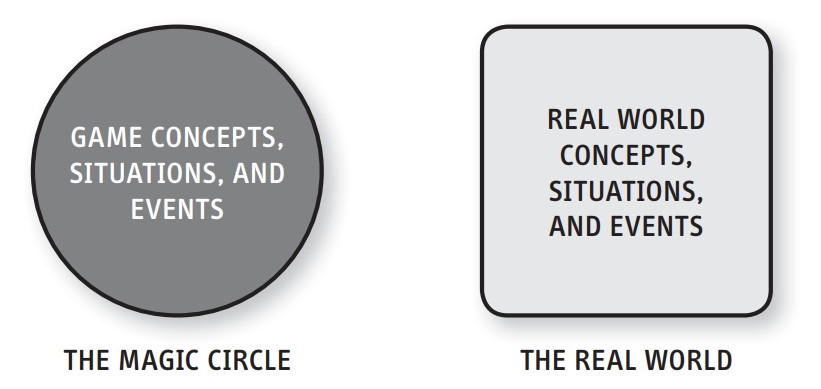
\includegraphics[width=\textwidth]{./Pictures/res/fundamentals/magic-circle}
    \caption{Magic Circle \cite{10.5555/2544002}}
    \label{fig:magic-circle}
\end{figure}
\\
\textbf{Goals} need to be set in order to correctly design and implement a game.
During the play-through, there always have to be objectives to the user.
Even though a game may seem very goalless, there may be some unseen goals such as acts of creativity / creation, which may also be
referred to as a goal.
\\
\textbf{Rules} instruct the player through the game and give a boundary or limit to the game.
They are used to describe allowed actions during the gameplay, define progression and - if applicable - give a condition to
end the game.
\\ \\
Generally, the definition of a game is very broad and there are different opinions on the definition, however most of them
do not refer to the games' purpose: it may be purely for entertainment, but can also be for studying, training or attracting interest
for a topic, which is especially the case in the scope of this work.

\subsection{Educational Games}\label{subsec:educational-games}
Most games have a certain factor of education, so called \textit{stealth-education} involved, even though not
specifically intended to be educational.
However, there exist also games with the specified purpose of education, this may include simulations, persuasive games,
games for studying and games that support health and growth.
Educational games are a sub-genre of the \textit{Serious Games}-genre and aim to present or solve real world problems,
while maintaining a factor of entertainment.
Different ways of presentation may be used for educational games~\cite[p.43]{10.5555/2544002}.

\subsection{Game Engines}\label{subsec:game-engines}
Game engines are software frameworks that game developers use to create video games more efficiently.
They provide a set of tools and features that allow developers to create games without needing to build everything from scratch.
Game engines typically provide a range of features, including graphics rendering, physics simulation, audio processing, animation, scripting, and networking.
\\
Game engines come in various forms, from open-source engines that can be freely used and modified by anyone, to commercial engines that require a license fee to use.
Some examples of popular game engines include Unity, Unreal Engine, CryEngine, and GameMaker Studio.
\\
Game engines can help reduce the time and cost of game development by providing pre-built components and tools, allowing developers to focus on creating the game's content and gameplay mechanics instead of building the underlying technology.
Additionally, game engines can make it easier to create games that run on multiple platforms, such as desktop computers, mobile devices, and gaming consoles, by providing cross-platform support.
\\
Game engines have become an essential part of the game development process, and have helped democratize game development by making it more accessible to independent developers and small studios.


\subsection{Entity Component System}\label{subsec:entity-component-system}
For the game engine, a generic entity component system (ECS) design pattern is used.
The basic idea behind using an ECS is to separate object data and behavior into components, respectively systems.
Each entity is a unique identifier for an object within the game, this can be anything from a button to a sound.
Entities consist of a variety of components, while each entity can have different components based on the needs.
A purely graphical entity which shows an image may only consist of a single graphics component, however another entity may contain
a component for graphics, one for sound and another one that holds collision information.
It is important to note, that components never change an entities' behavior, but only contain data that describes the entity.
Systems are responsible for collecting all relevant entities (i.e.\ entities that contain specific components) and processing them.
An example for a system is a rendering engine, which collects all graphical entities \& components and renders them to the screen by
using the data that is stored within the respective graphics components.
\\
There are different approaches on the implementation of Entity Component Systems, and they may be combined with other programming
patterns.
\section{System Design}\label{sec:system-design}
The process of aircraft system design involves multiple stages, starting with requirements gathering.
During this stage, the design team gathers information about the intended use of the aircraft, the desired performance goals, and any relevant safety and environmental regulations.
This information is used to define the design requirements for the aircraft system.
\\
Once the requirements are defined, the design team moves on to the conceptual design stage.
Here, they develop initial design concepts that meet the requirements defined in the first stage.
These concepts may involve trade-offs between different design factors such as weight, cost, and performance.
\\
After the conceptual design stage, the design team moves on to the preliminary design stage.
During this stage, the design concepts are refined and evaluated in greater detail.
The team may use computer simulations and testing to assess the performance of the aircraft system under different conditions.
\\
Once the preliminary design is complete, the detailed design stage begins.
During this stage, the team creates detailed designs for each component of the aircraft system, such as the propulsion system, avionics, and control systems.
These detailed designs must meet the requirements defined in the first stage and be compatible with the other components of the system.
\\
After the detailed design stage, the manufacturing stage begins.
During this stage, the aircraft system components are manufactured and assembled into the final aircraft.
The manufacturing process may involve multiple rounds of testing and quality control to ensure that the aircraft system is safe, reliable, and meets the design requirements.
\\
Finally, the aircraft system is tested and evaluated during the flight test stage.
Flight testing is critical to validating the performance of the aircraft system in real-world conditions and identifying any issues that need to be addressed before the aircraft is certified for operation.
Once the flight testing is complete, the aircraft system is ready for use in commercial or military applications.
\subsection{Failure Probability}\label{subsec:failure-probability}
The probability of a failure of a system during a specified point in time is defined as~\cite{lfs2}:
\begin{equation}
    \label{eq:failure-probability}
    P_f(t) \in [0,1]
\end{equation}
\subsection{Reliability}\label{subsec:reliability}
Reliability defines the probability of a working system at a specified point in time,
therefore it is the inverse of the failure probability~\cite{lfs2}:
\begin{equation}
    \label{eq:reliability}
    P_k(t) = 1 - P_f(t) \in [0,1]
\end{equation}
\subsection{Integrity}\label{subsec:integrity}
The detection probability of an error in a system is defined as integrity~\cite{lfs2}:
\begin{equation}
    \label{eq:integrity}
    C \in [0,1]
\end{equation}
\subsection{Safety Effect}\label{subsec:safety-effect}
There exist different categories of safety effects in the CS-25 for aircraft certification that define the requirements to different systems.
A mapping of safety effect to minimum failure probability has to be achieved in order to successfully certify aircraft systems.
The below table~\ref{tab:safety-effect} displays the different categories.

\begin{table}[!htb]
    \centering
    \begin{tabular}{l|l|l}
        Safety Effect    & Safety Effect short & Accepted Failure Probability \\ \hline
        Catastrophic     & CAT                 & $P_f(1h) <= 10e-9$           \\
        Hazardous        & HAZ                 & $P_f(1h) <= 10e-7$           \\
        Major            & MAJ                 & $P_f(1h) <= 10e-5$           \\
        Minor            & MIN                 & $P_f(1h) <= 10e-3$           \\
        No Safety Effect & NSE                 & $P_f(1h) < 1$
    \end{tabular}
    \caption{Definition of safety effect categories}
    \label{tab:safety-effect}
\end{table}
\section{Redundancy Concepts}\label{sec:redundancy-concepts}
By default, the failure probability of integrated components is defined as $10e-4$, which means, that with only a single component
safety effect requirements of categories higher than \textit{Major} are out of scope.
Therefore, different redundancy concepts have been developed and are being used in system architectures.
These include duplex, triplex and quadruplex systems - meaning, a component is replicated multiple times to run the same program.
One needs to divide between replicated computers, also called \textbf{channels}, and replicated components (e.g.\ CPU) within a computer,
namely \textbf{lanes}.
It is important to note, that each lane or channel is merged right before an actuator.
The decision on how the actuator needs to move is done by a \textbf{voting} component, which can have different methods of voting
for the correct output: mean value, median value, democratic decision.
The voting component generally is the bottleneck of aircraft systems and needs to guarantee a low probability of failure
due to being the most critical component in the chain, since all further movement is based on its decision.
Actuators can also have a monitoring component, which ensures the correct movement of itself.
This is called a \textbf{Com-Mon} - Command \& Monitoring - system.
It negatively affects the failure probability, but the integrity, meaning that the system is able to react to a possible failure due
to noticing it.
A number of different concepts is shown in the figures below, which also serves as a guideline to the level design of the game,
since the presentation and understanding of exactly these concepts is the core of the game.
\subsection{Safety Analysis}\label{subsec:safety-analysis}

\section{Markov Process}\label{sec:markov-process}
The aircraft design process generally has to comply with the requirements that are stated in regulatory files such as the FAR 25
in order to qualify for the aircraft certification documents.
There are different guidelines for the conduction of the safety assessment process for aircraft systems, which include the
recommendation of quantitative analysis methods such as Fault Tree Analysis, Dependence Diagrams and Markov Analysis.
While the most widely used method today is the Fault Tree Analysis~\cite{7447967}, the Markov Analysis is used for the backend
part of this work and will therefore be explained in detail.

A Markov process, also called Markov chain, is a mathematical model describing a system that changes over time.
Future states of the model are determined only by its current state and by the transition probability, not taking into account
the former states. \todo{add source}

\subsection{States}\label{subsec:states}
Possible states for the system design Markov model include the correct state and different failure states, such as out of control
or passive failures.
Each failure can also be of a different kind, e.g.\ a mechanical failure has a different probability than a loss of electrical power.

